\documentclass{ximera}

\usepackage{todonotes}

\newcommand{\RR}{\mathbb R}
\renewcommand{\d}{\,d}
\newcommand{\dd}[2][]{\frac{d #1}{d #2}}
\renewcommand{\l}{\ell}
\newcommand{\ddx}{\frac{d}{dx}}
\newcommand{\dfn}{\textbf}
\newcommand{\eval}[1]{\bigg[ #1 \bigg]}
\renewcommand{\epsilon}{\varepsilon}
\newcommand{\p}[1]{\left(#1\right)}
\newcommand{\br}[1]{\left[#1\right]}
\newcommand{\set}[1]{\left\{#1\right\}}


\let\prelim\lim
\renewcommand{\lim}{\displaystyle\prelim}

\colorlet{textColor}{black} 
\colorlet{background}{white}
\colorlet{penColor}{blue!50!black} % Color of a curve in a plot
\colorlet{penColor2}{red!50!black}% Color of a curve in a plot
\colorlet{penColor3}{red!50!blue} % Color of a curve in a plot
\colorlet{penColor4}{green!50!black} % Color of a curve in a plot
\colorlet{penColor5}{orange!80!black} % Color of a curve in a plot
\colorlet{fill1}{blue!50!black!20} % Color of fill in a plot
\colorlet{fill2}{blue!10} % Color of fill in a plot
\colorlet{fillp}{fill1} % Color of positive area
\colorlet{filln}{red!50!black!20} % Color of negative area
\colorlet{gridColor}{gray!50} % Color of grid in a plot


\newcommand{\fullwidth}{}
\newcommand{\normalwidth}{}



%% makes a snazzy t-chart for evaluating functions
\newenvironment{tchart}{\rowcolors{2}{}{background!90!textColor}\array}{\endarray}


\author{Gregory Hartman \and Matthew Carr}
\license{Creative Commons 3.0 By-NC}
\acknowledgement{https://github.com/APEXCalculus}

\begin{document}

\begin{exercise}

\outcome{Evaluate the limit as $x$ approaches a point where there is a vertical asymptote.}
\outcome{Identify when a limit does not exist.}


\tag{limit} 
\tag{discontinuous}
\tag{vertical asymptote}

  Find 
  \[
  \lim_{x\to 2} \left({\frac{x^2+7x+10}{x^2-4x+4}}\right)
  \begin{prompt}
  = \answer{\text{DNE}}.
  \end{prompt}
  \]
    \begin{hint}
     This function is \underline{not} continuous everywhere, but both the numerator and denominator are continuous everywhere as functions. Thus, if the limit of $\frac{x^2+7x+10}{x^2-4x+4}$ as $x\to{a}$ does not exist, then the denominator $x^2-4x+4$ must be zero at $a$. Does $x^2-4x+4=0$ when $x=2$? Does $x^2+7x+10=0$ at $x=2$ as well?
    \end{hint}
     \begin{hint}
    	Take a look at the graph of the function
    \begin{center}
     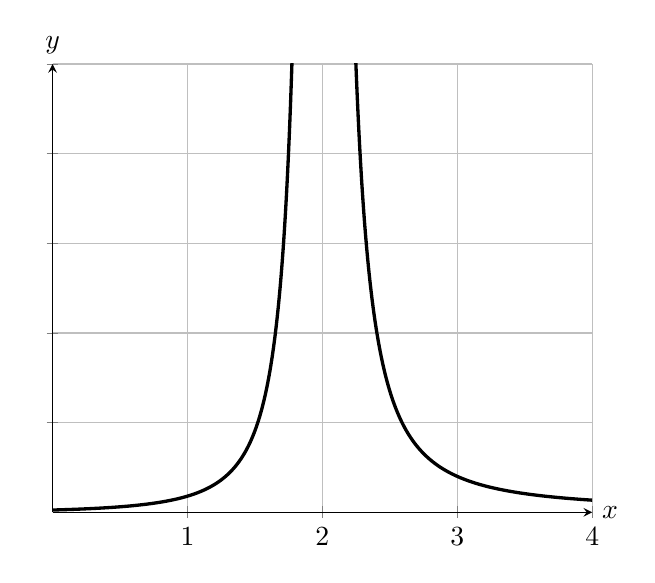
\begin{tikzpicture}
	\begin{axis}
	[ymin=0,ymax=500, axis lines=center,xlabel=$x$,ylabel=$y$,every axis y 
	label/.style={at=(current axis.above origin),anchor=south},every axis x label/.style={at=(current axis.right of origin),anchor=west},
	domain=0:4,
	yticklabels={},
	ymajorgrids=true,
	grid = major
	]
	\addplot[domain=0:197/100,very thick,smooth,samples=600]
	{(\x^2+7*\x+10)/(\x^2-4*\x+4)};
	\addplot[domain=203/100:4,very thick,smooth,samples=600]
	{(\x^2+7*\x+10)/(\x^2-4*\x+4)};
	\end{axis}
       \end{tikzpicture}      
      \end{center} 
      Apply the limit law which says that, if both $\lim_{x\to a}f(x)$ and $\lim_{x\to a}g(x)$ exist, then, if $\lim_{x\to a}g(x)\ne0$, $\lim_{x\to{a}}\frac{f(x)}{g(x)}=\frac{\lim_{x\to a}f(x)}{\lim_{x\to{a}}g(x)}$. Observe what happens around (but not at) $x=2$.
    \end{hint}
    \begin{hint}
    First, notice that the quadratic equation gives only one solution to $x^2-4x+4=0$, namely $x=2$. Therefore, $x^2-4x+4=\left({x-2}\right)^2$. Since the factorization of $x^2+7x+10$ does not contain two factors of $\left({x-2}\right)$, there is a discontinuity at $x=2$. On the one hand, for $x>-2$, $x^2+7x+10>0$ and for all $x$, $x^2-4x+4>0$ (this latter result follows as the quadratic formula tells us that $x^2-4x+4=0$ only at $x=2$, so $x^2-4x+4=\left({x-2}\right)^2$, and as we know, squared numbers are always positive); hence, for $x>-2$, $\frac{x^2+7x+10}{x^2-4x+4}>0$. On the other hand, for every number $a$ satisfying $-2<a<2$ or $a>2$, the limit $\lim_{x\to a}\frac{x^2+7x+10}{x^2-4x+4}$ exists because both the numerator and the denominator are continuous and nonzero for all $x$ satisfying $-2<x<2$ or $x>2$. Applying several limit laws tells us that $\lim_{x\to a}\left({x^2+7x+10}\right)=\left({\lim_{x\to a}(x)}\right)^2+7\cdot\lim_{x\to a}(x)+\lim_{x\to a}\left({10}\right)=a^2+7a+10$ and $\lim_{x\to a}\left({x^2-4x+4}\right)=\left({\lim_{x\to a}(x)}\right)^2-4\cdot\lim_{x\to a}(x)+\lim_{x\to a}\left({4}\right)=a^2-4a+4$. Hence, as both limits of the preceeding functions exist and $a^2-4a+4\ne0$, for  $-2<a<2$ or $a>2$, $\lim_{x\to a}\left({\frac{x^2+7x+10}{x^2-4x+4}}\right)=\frac{\lim_{x\to a}\left({x^2+7x+10}\right)}{\lim_{x\to a}\left({x^2-4x+4}\right)}=\frac{a^2+7a+10}{a^2-4a+4}$.
    
    Combining these observations with the fact that the denominator becomes arbitrarily close to $0$ as $a$ approaches $2$, while the numerator approaches $28$, we see that $\lim_{x\to 2}\left({\frac{x^2+7x+10}{x^2-4x+4}}\right)=\infty$, because, from both sides of $x=2$, $\frac{x^2+7x+10}{x^2-4x+4}$ approaches $\infty$.
 \end{hint}
\end{exercise}

\end{document}